\documentclass[a4paper,11pt]{jsarticle}

% 数式
\usepackage{amsmath,amsfonts}
\usepackage{bm}
% 画像
\usepackage[dvipdfmx]{graphicx}
% bibTeX
\usepackage[backend = biber,style =apa, sorting =none,]{biblatex}

% 参考文献ファイルのリスト
\addbibresource{references.bib}

% 等式番号を章ごとに割り振る
\makeatletter
\@addtoreset{equation}{section}
\def\theequation{\thesection.\arabic{equation}}
\makeatother

\begin{document}

\title{計算機科学実験2ソフトウェア報告書1}
\author{2021年度入学 学籍番号:1029-33-1415 安済翔真}
\date{\today}
\maketitle

\section*{ステージパラメータ}
\subsection*{setLevelDifficulty}
ステージのレベルを変更した。デフォルトのレベルが最低レベルであるレベル0である
ということがわかった。レベル0ではファイアとジャンプを繰り返しながら一直線に走っていくだけでクリアできたのに対し、
レベル3では飛びながら襲ってくる敵や落とし穴が現れて単純なコードではクリアできなくなっていた。

\begin{figure}[h]
  \centering
  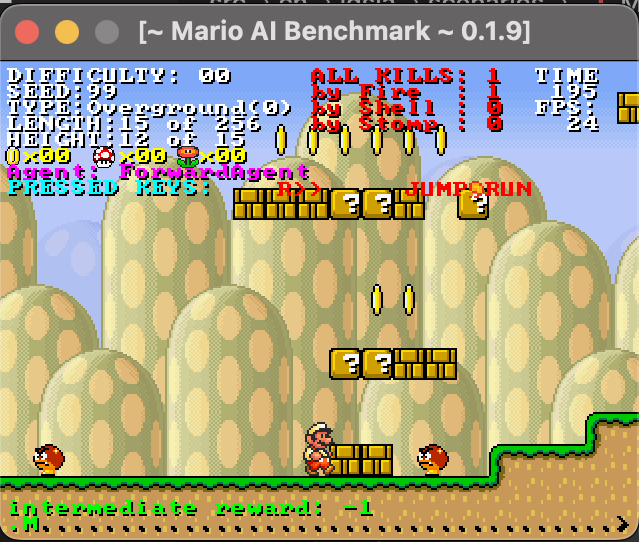
\includegraphics[scale=0.6]
    { images/report1/image-diff0.png }
  \caption[]{Difficulty = 0の時のステージ}
\end{figure}

\begin{figure}[h]
  \centering
  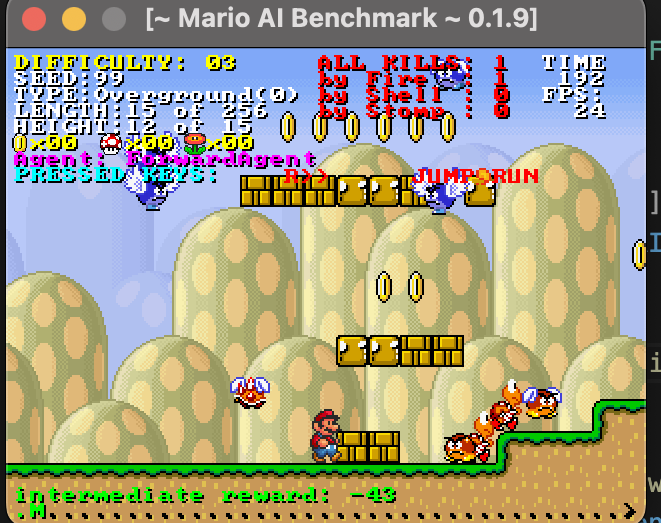
\includegraphics[scale=0.6]{
    images/report1/image-diff3.png
  }
  \caption[]{Difficulty = 3の時のステージ}
\end{figure}


\subsection*{setBlocksCount}
setBlocksCountをfalseにしてブロックがないステージを試した。
ブロックがないため単調なステージとなっていたが、
敵にぶつかって死ぬことが何度かあった。

\begin{figure}[h]
  \centering
  \includegraphics*[scale=0.6]{
    images/report1/image-no-block.png
  }
  \caption[]{ブロックを無くした場合のステージ}
\end{figure}

\subsection*{setFlatLevel}
setFlatLevelをtrueにして地面が平らなステージを試した。
ブロックがないステージよりもさらに単調なステージとなったが、
ファイアボールを打ってジャンプをしながら進んでいくだけで
クリアできるステージになった。

\begin{figure}
  \centering
  \includegraphics*[scale=0.6]{
    images/report1/image-flat-stage.png
  }
  \caption[]{地面を平らにした場合のステージ}
\end{figure}

\section*{すでに実装されているエージェント}
ForwardAgentの実装を確認した。

\subsection*{reset}
actionを要素数:Environment.numberOfKeysの配列として初期化し、右ボタンとダッシュボタンを
押した状態にしている。また、trueJumpCounterとtrueSpeedCounterを0にしている。

\subsection*{DangerOfAny}
マリオの前方に壁があるか、マリオの前方足元に穴があるか、前方に敵がいる場合にtrueを返す。

\subsection*{getAction}
DangerOfAnyがtrueで、前方にあるのがコインではない場合にジャンプを行う。また、ジャンプをしている状態
が16チック以上続いた場合もジャンプを止めるようになっている。


\printbibliography[title=参考文献]

\end{document}
